\documentclass[11pt]{article}

\usepackage[spanish]{babel}
\usepackage{translations}
\usepackage[titles]{tocloft}
\usepackage{multicol}
\usepackage{graphicx}
\usepackage{amsmath}
\usepackage{hyperref}
\usepackage{amsmath}
\usepackage{amssymb}
\usepackage{listings}
\usepackage{courier}
\usepackage[margin=1in]{geometry}
\usepackage{changepage}
\usepackage{titlesec}
\usepackage{wrapfig}
\usepackage[version=4]{mhchem}
\usepackage{multirow}
\usepackage{siunitx}
\usepackage{ragged2e}
\usepackage{adjustbox}
\usepackage[font=small,labelfont=bf]{caption}
\usepackage[table,xcdraw]{xcolor}
\usepackage{afterpage}
\usepackage{xfrac}
\usepackage{animate}
\usepackage{subcaption}
\usepackage{tcolorbox}
\usepackage{nicefrac}

\setlength{\parindent}{1cm}

\definecolor{mytheoremfr}{HTML}{7B0000}
\definecolor{mytheorembg}{HTML}{f5e4e1}

\tcbuselibrary{theorems,skins,hooks}
\newtcbtheorem[number format=\alph]{Theorem}{Pregunta}
{%
	enhanced,
	colback = mytheorembg,
	frame hidden,
	boxrule = 0sp,
	borderline west = {2pt}{0pt}{mytheoremfr},
	sharp corners,
	detach title,
	before upper = \tcbtitle,
	coltitle = mytheoremfr,
	fonttitle = \bfseries\sffamily,
	description font = \mdseries,
	separator sign none,
	segmentation style={solid, mytheoremfr},
}
{th}

\usetikzlibrary{arrows,calc,shadows.blur}
\tcbuselibrary{skins}
\newtcolorbox{note}[1][]{%
	enhanced jigsaw,
	colback=gray!10!white,%
	colframe=gray!80!black,
	size=small,
	boxrule=1pt,
	title=\textbf{Ejercicio:},
	halign title=flush center,
	coltitle=black,
	drop shadow=black!50!white,
	attach boxed title to top left={xshift=1cm,yshift=-\tcboxedtitleheight/2,yshifttext=-\tcboxedtitleheight/2},
	minipage boxed title=2.5cm,
	boxed title style={%
			colback=white,
			size=fbox,
			boxrule=1pt,
			boxsep=2pt,
			underlay={%
					\coordinate (dotA) at ($(interior.west) + (-0.5pt,0)$);
					\coordinate (dotB) at ($(interior.east) + (0.5pt,0)$);
					\begin{scope}[gray!80!black]
						\fill (dotA) circle (2pt);
						\fill (dotB) circle (2pt);
					\end{scope}
				},
		},
	#1,
}

\newcommand{\preguntaAlaMadreDeRocio}[1]{\begin{Theorem}{#1}{}\end{Theorem}}
\newcommand{\laputa}[1]{\begin{note}{#1}{}\end{note}}

\renewcommand{\labelenumi}{\alph{enumi}.}
   
\newcommand{\titulo}{Análisis y Diseño de\\ Sistemas Ópticos \\\ \\(Práctica 2)}
\newcommand{\nombreestudiante}{Víctor Mira Ramírez\\ Rocío Ponsoda Orgilés}
\newcommand{\nombredirector}{Celia García Llopis}
\newcommand{\fecha}{\date{Diciembre 2023}}

\pagebreak

\renewcommand{\listtablename}{Índice de tablas} 
\renewcommand{\tablename}{Tabla} 
\renewcommand\cftsecdotsep{\cftdotsep}

\setlength{\cftbeforesecskip}{0.5ex}
\renewcommand{\cftsecfont}{%
  \fontsize{11}{13}\usefont{OT1}{phv}{bc}{n}\selectfont
}
\makeatletter
\renewcommand{\@pnumwidth}{1.75em}
\renewcommand{\@tocrmarg}{2.75em}
\makeatother

\begin{document}

    \begin{titlepage}
    	\centering
    	
\includegraphics[width=65mm]{fotos/logoUA.png}\par
    	\vspace{1cm}
    	{\huge\bfseries \vspace{15mm} \titulo \par}
    	\vfill
    	{\large 
    	\vfill
    	Estudiantes:\par\vspace{2mm}
    	\nombreestudiante\par
    	\vfill
    	Profesora:\par\vspace{2mm}
        \nombredirector
        \vfill
        Universidad de Alicante\par
        Facultad de Ciencias: Departamento de Óptica, Farmacología y Anatomía\par
        Óptica I\par
    	\fecha\par}
    \end{titlepage}
    
    \clearpage

    \begin{abstract}\label{sec:abstract}
        %% PROPUESTA DE ABSTRACT %%
        En esta práctica presentamos una introducción general a los programas de análisis y diseño de elementos ópticos. En concreto nos familiarizaremos con el programa \textit{OSLO EDU} y sus posibilidades más básicas. Construiremos un sistema con dos lentes del cual obtendremos los resultados a las cuestiones propuestas en clase.
    \end{abstract}\vspace{0.3cm}  
    
    \section*{Cuestiones propuestas}

        \laputa{Construir un sistema de lentes (puede ser con una lente pero se valorará un sistema con dos o tres lentes) y realizar los siguientes cálculos:}

        \noindent En nuestro caso vamos a usar un sistema de dos lentes que seleccionaremos del catálogo del programa. Las características de dichas lentes las recogemos en la siguiente tabla:
        \begin{table}[ht]
            \centering
            \begin{tabular}{c|cc|cc|}
                \cline{2-5}
                \multicolumn{1}{l|}{}                    & \multicolumn{2}{c|}{Lente 1 (planocóncava)}      & \multicolumn{2}{c|}{Lente 2 (biconvexa)}         \\ \cline{2-5} 
                \multicolumn{1}{l|}{}                    & \multicolumn{1}{c|}{Superficie 1} & Superficie 2 & \multicolumn{1}{c|}{Superficie 3} & Superficie 4 \\ \hline
                \multicolumn{1}{|c|}{Radio (mm)}         & \multicolumn{1}{c|}{$-46.008$}    & $0$          & \multicolumn{1}{c|}{$45.124$}     & $-45.124$    \\ \hline
                \multicolumn{1}{|c|}{e (mm)}             & \multicolumn{1}{c|}{$2$}          & $10$         & \multicolumn{1}{c|}{$5.5$}        & $100$        \\ \hline
                \multicolumn{1}{|c|}{$\varnothing$ (mm)} & \multicolumn{1}{c|}{$12.3$}       & $12.3$       & \multicolumn{1}{c|}{$11.25$}      & $11.25$      \\ \hline
                \multicolumn{1}{|c|}{n}                  & \multicolumn{2}{c|}{$1.46$}                      & \multicolumn{2}{c|}{$1.46$}                      \\ \hline
            \end{tabular}
            \caption{Lentes utilizadas}
        \end{table}\\

        \noindent En el programa \textit{OSLO} estos datos los hemos introducido de forma que se obtiene el sistema óptico que representamos a continuación.
        \begin{figure}[ht]
            \centering
            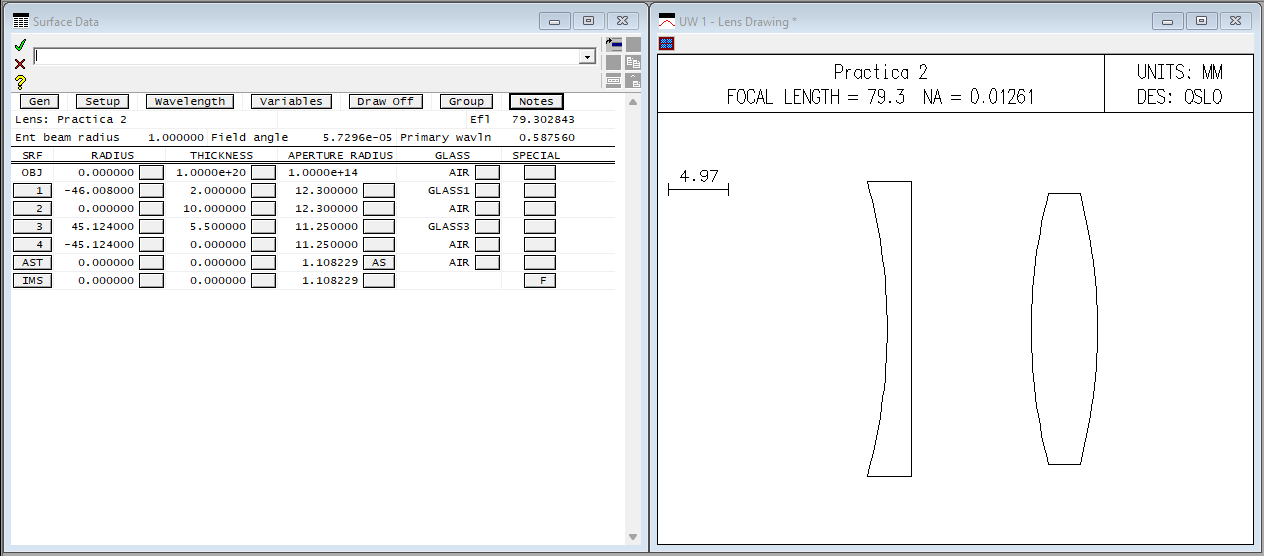
\includegraphics[width=\textwidth]{fotos/datoslentes+lente.png}
            \caption{Sistema óptico}
            \label{fig:proyecto}
        \end{figure}
    
        \clearpage
        %    A
        \preguntaAlaMadreDeRocio{Calcula la focal de la lente y la posición de los planos principales y focales.}
        
        \noindent La focal de la lente es calculada por el propio programa. En la figura (\ref{fig:proyecto}) aparece en la ventana de la izquierda, \textit{Surface Data}, donde podemos observar cómo en la parte superior derecha de la ventana hay un apartado llamado \textit{Efl} que nos indica la focal. Para el caso de nuestro sistema, la focal es de $f = 79.3\ mm$.\\

        \noindent Para obtener la posición de los planos principales y focales nos fijamos en la ventana \textit{Paraxial Setup} que observamos en la figura (\ref{fig:paraxial_setup})

        \begin{figure}[ht]
            \centering
            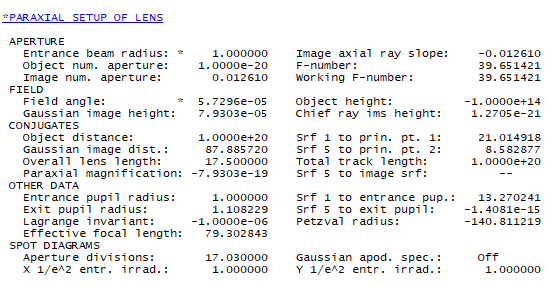
\includegraphics[width=0.8\textwidth]{fotos/paraxial.png}
            \caption{\textit{Paraxial Setup}}
            \label{fig:paraxial_setup}
        \end{figure}

        \noindent En el apartado \textit{CONJUGATES} podemos observar dichas posiciones, la distancia del plano principal objeto a la primera superficie será de $21.00\ mm$ (\textit{Srf 1 to prin. pt. 1}) mientras que la distancia del plano principal imagen a la segunda superficie será de $8.58\ mm$ (\textit{Srf 5 to prin. pt. 2}). Nótese que como ambos valores son positivos, representan distancias hacia la derecha.\\

        \noindent Para calcular los planos focales haremos servir el dato de la focal del sistema que hemos obtenido previamente, obteniendo que el plano focal objeto estará a $58.3\ mm$ a la izquierda de la primera superficie mientras que el plano focal imagen estará a $87.88\ mm$ de la segunda superficie.

        \[
        f=79.3 \Longrightarrow 
        \left\{\begin{aligned}
            &F=H-f=21-79.3=-58.3\\
            &F^\prime=H^\prime+f=8.58+79.3=87.88\\
        \end{aligned}\right.
        \]

        A modo de resumen:
        \begin{table}[ht]
            \centering
            \begin{tabular}{|cc|cc|}
                \hline
                \rowcolor[HTML]{010066} 
                \multicolumn{2}{|c|}{\cellcolor[HTML]{010066}{\color[HTML]{EFEFEF} Plano principal ($mm$)}} &
                  \multicolumn{2}{c|}{\cellcolor[HTML]{010066}{\color[HTML]{EFEFEF} Plano focal ($mm$)}} \\ \hline
                \rowcolor[HTML]{CBCEFB} 
                \multicolumn{1}{|c|}{\cellcolor[HTML]{CBCEFB}\begin{tabular}[c]{@{}c@{}}Objeto (\textit{respecto} \\ \textit{a la 1a sup.})\end{tabular}} &
                  \begin{tabular}[c]{@{}c@{}}Imagen (\textit{respecto}\\ \textit{a la 2a sup.})\end{tabular} &
                  \multicolumn{1}{c|}{\cellcolor[HTML]{CBCEFB}\begin{tabular}[c]{@{}c@{}}Objeto (\textit{respecto} \\ \textit{a la 1a sup.})\end{tabular}} &
                  \begin{tabular}[c]{@{}c@{}}Imagen (\textit{respecto}\\ \textit{a la 2a sup.})\end{tabular} \\ \hline
                \multicolumn{1}{|c|}{$21.0$} &
                  $8.58$ &
                  \multicolumn{1}{c|}{$-58.3$} &
                  $87.88$ \\ \hline
            \end{tabular}
            \caption{Planos principales y focales}
            \label{tab:planos principales y focales}
        \end{table}
        
        \clearpage
        %   B
        \preguntaAlaMadreDeRocio{Representa mediante el OSLO el trazado de rayos de este sistema para tres haces (uno que pasa por el extremo, un segundo a la mitad mm y un tercero a $0,5\ mm$).}
        \begin{wrapfigure}[11]{l}{0.6\textwidth}
            \vspace{-0.5cm}
            \centering
            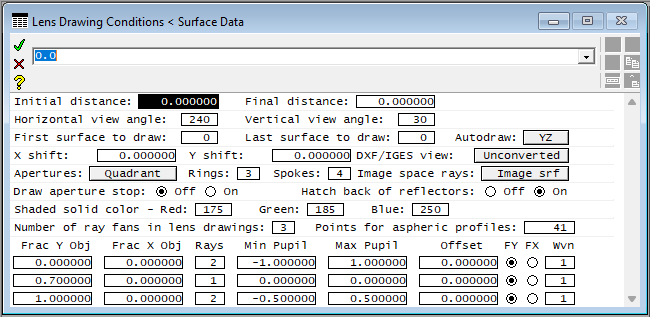
\includegraphics[width=0.6\textwidth]{fotos/apartadob_preparación.png}
        \end{wrapfigure}
        
        \noindent Para hacer la representación pertinente de los rayos vamos a modificarlos desde el menú \textit{OPC: Edit Lens Drawing Conditions}. Nos hemos de asegurar tanto de que los rayos van a ir a parar al plano imagen como de que introducimos el tamaño de nuestras lentes para limitar su paso. \\
        
        \begin{wrapfigure}[4]{r}{0.6\textwidth}
            \vspace{-0.5cm}
            \centering
            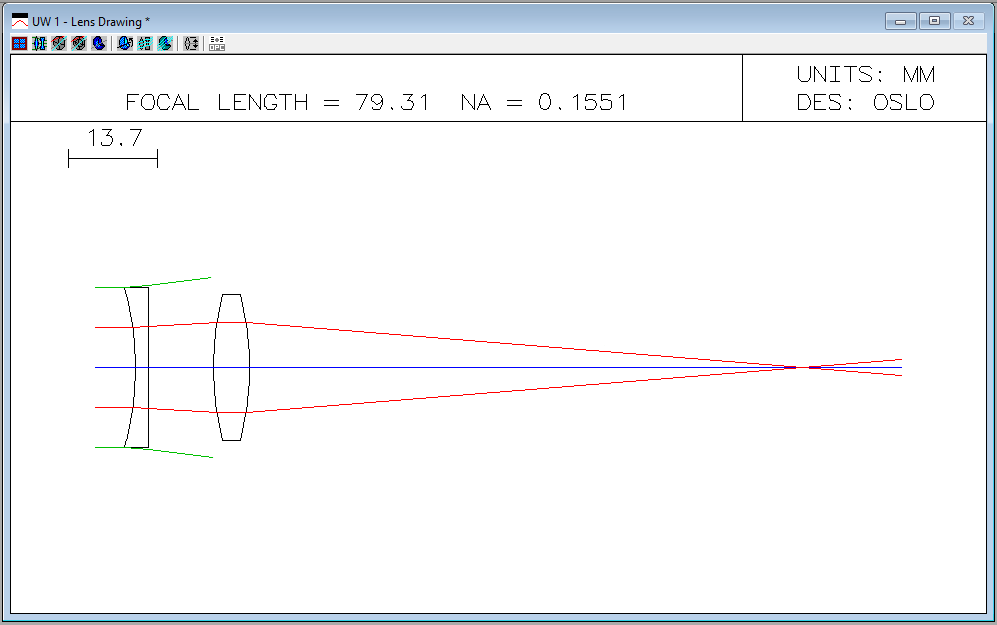
\includegraphics[width=0.6\textwidth]{fotos/apartadob.png}
        \end{wrapfigure}

        \noindent Una vez hemos preparado de esta forma nuestra representación vemos que el trazado con tres rayos queda de la siguiente forma:\\\hspace{0cm}\\\hspace{0cm}\\\hspace{0cm}\\\hspace{0cm}\\\hspace{0cm}\\\hspace{0cm}\\\hspace{0cm}\\\hspace{0cm}\\

        %  C
        \preguntaAlaMadreDeRocio{Utiliza el setup como calculadora paraxial y calcula la posición de la imagen y el aumento para una posición del objeto distinto del infinito.}
        \noindent Hasta el momento hemos considerado que el objeto que usamos para estudiar este sistema óptico se encuentra en el infinito. Ahora vamos a cambiar de forma manual su posición, tomándola de forma que la distancia entre el objeto y el plano principal objeto (PP1) sea $a = -100\ mm$.\\
        
        \begin{wrapfigure}[10]{l}{0.6\textwidth}
            \vspace{-0.6cm}
            \centering
            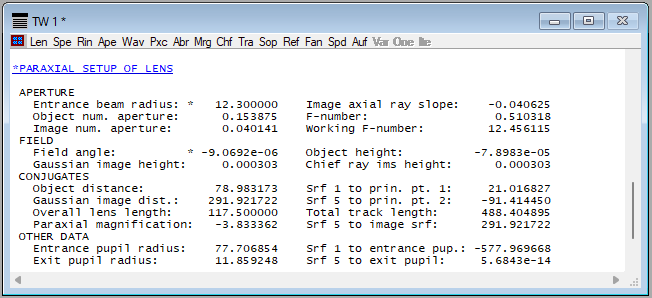
\includegraphics[width=0.6\textwidth]{fotos/paraxial_setup_apartadoc.png}
        \end{wrapfigure}
        \noindent En la sección \textit{Conjugates} de esta imagen se puede ver la distancia entre objeto, imagen y planos principales. Vemos que en este caso, la distancia entre la imagen y el plano principal imagen (PP2), magnitud que reconocemos por el nombre de \textit{Gaussian image dist} es $a' = 291.92\ mm$.\\
        
        \noindent El aumento lateral del sistema óptico nos viene dado por \textit{Paraxial magnification} y corresponde a $\beta = -3.83$. A nivel óptico, esto implica que la imagen se verá mayor a invertida al objeto.

        %  D
        \preguntaAlaMadreDeRocio{Estudia las aberraciones de este sistema AEL siguiendo los pasos de la práctica.}
        \noindent La AEL (Aberración Esférica Longitudinal) es la aberración relacionada con la distancia que tenemos entre el punto de corte de los rayos en el eje óptico y el plano focal paraxial. Para estudiarla en nuestro sistema óptico, vamos a tomar varios casos donde el rayo considerado no esté a la altura máxima. Conseguiremos además una serie de gráficas que nos representen la AEL para este rango de alturas.\\ 

        \begin{wrapfigure}[9]{r}{0.6\textwidth}  
            \vspace{-1cm}
            \caption{AEL para un $100 \%$ de la altura máxima}
            \vspace{-0.2cm}
            \centering
            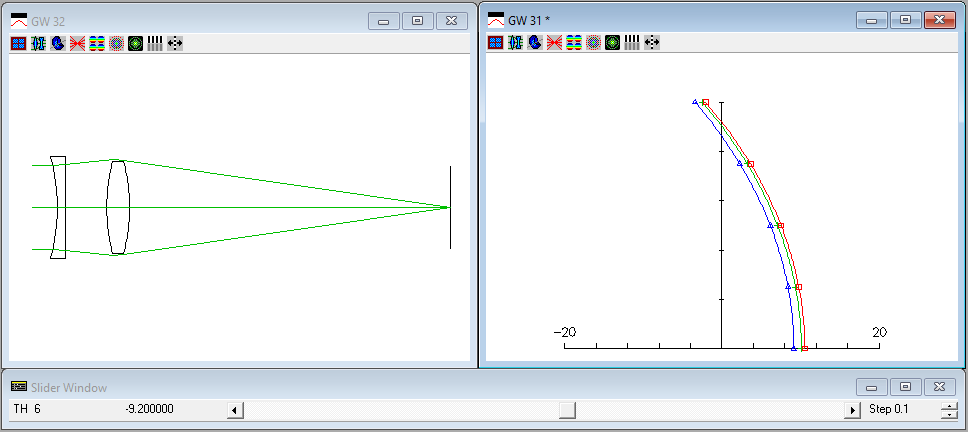
\includegraphics[width = 0.6\textwidth]{fotos/apartadod_1.png}
        \end{wrapfigure} 
        
        \noindent Partimos de la siguiente configuración para nuestro sistema, donde hemos tomado tres rayos que pasen por el máximo, el mínimo y el centro de la pupila:\\

        \noindent Ahora vamos hacer el mismo estudio, pero para alturas correspondientes al $80 \%$, $60 \%$, $40 \%$ y $20 \%$ de la altura máxima.
        
        \begin{figure}[h]
            \centering
            \subfloat[$80 \%$ altura máxima]{
            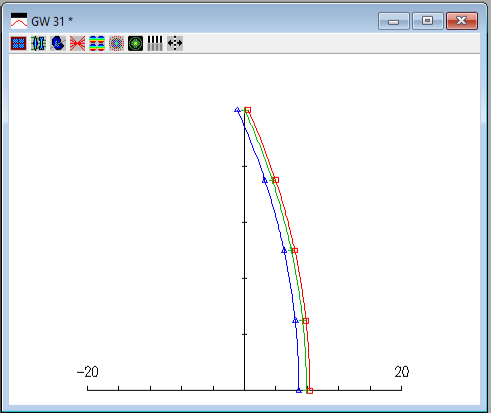
\includegraphics[width=0.308\textwidth]{fotos/apartadod_2.png}}
            \subfloat[$60 \%$ altura máxima]{
            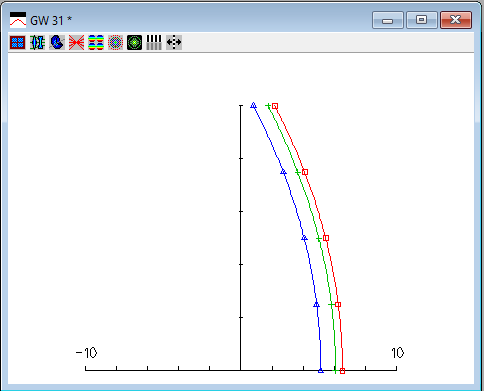
\includegraphics[width=0.32\textwidth]{fotos/apartadod_3.png}}
        \end{figure}
        \begin{figure}[h]
            \centering
            \subfloat[$80 \%$ altura máxima]{
            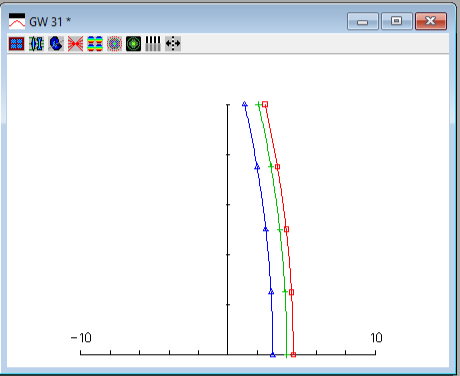
\includegraphics[width=0.31\textwidth]{fotos/apartadod_4.png}}
            \subfloat[$60 \%$ altura máxima]{
            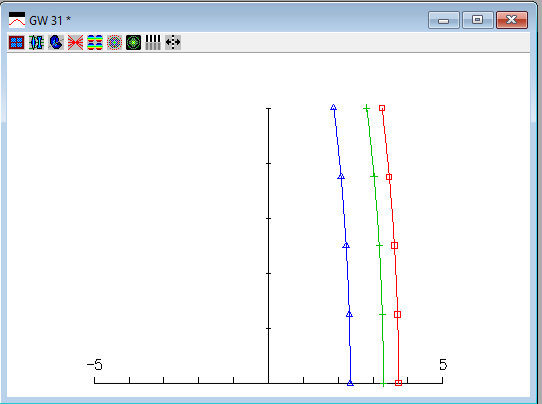
\includegraphics[width=0.34\textwidth]{fotos/apartadod_5.png}}
        \end{figure}

        \noindent En el siguiente cuadro incluimos los valores de la AEL para cada una de estas alturas, todo en unidades de $mm$.
        \begin{table}[h]
        \centering
            \begin{tabular}{|c|c|c|c|c|c|}
                \hline
                Altura   & $100 \%$ & $80 \%$ & $60 \%$ & $40 \%$ & $20 \%$ \\ \hline
                AEL      & $-9.2$   & $-7$    & $-5.2$  & $-3.1$  & $-2.4$  \\ \hline
            \end{tabular}
        \end{table}

        \clearpage
        %  E
        \preguntaAlaMadreDeRocio{Calcula cuál tendría que ser el radio de una o varias de las superficies de una de las lentes para que se minimice la aberración esférica y la focal sea la mitad del valor que se obtendría.}
        
        \noindent Como ya vimos en la primera práctica, para minimizar la aberración esférica hemos de variar el factor de forma de la lente. Para ello, vamos a hacer uso del programa \textit{OSLO} para facilitarnos los cálculos. Basta con proporcionar al programa qué queremos minimizar y las variables para lograrlo.\\

        \begin{wrapfigure}[13]{r}{0.55\textwidth}
            \vspace{-0.5cm}
            \centering
            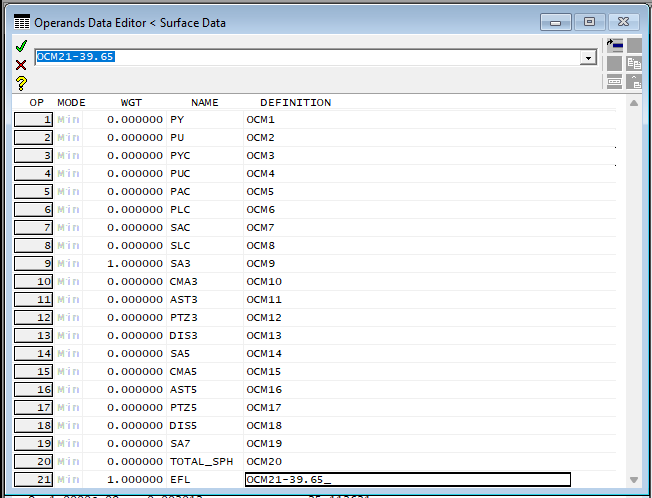
\includegraphics[width=0.55\textwidth]{fotos/operands.png}
        \end{wrapfigure}
        
        \noindent Para ello hemos de ir a la pestaña donde pone \textit{Optimize} $\to$ \textit{Generate error function} $\to$ \textit{Aberration Operands}, y allí cambiaremos a $1$ las variables que queremos minimizar: 
        \begin{itemize}
            \item Aberración Óptica de tercer orden (\textit{SA3})
            \item Focal efectiva (\textit{EFL})
        \end{itemize}
        
        \noindent Para conseguir que esta última sea la mitad del valor que se obtendría, hemos de centrar EFL en la mitad de nuestra focal del sistema, es decir, en \textit{OCM21} - $\nicefrac{f}{2}$.\\ \hspace{0cm}\\

        \begin{wrapfigure}[17]{l}{0.55\textwidth}
            \vspace{-0.5cm}
            \centering
            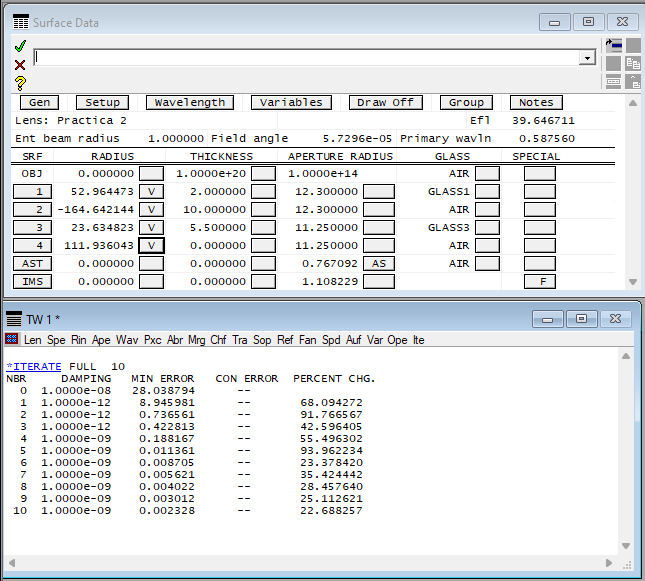
\includegraphics[width=0.53\textwidth]{fotos/radiosVariable.png}
        \end{wrapfigure}
        
        \noindent Ahora, hemos de decirle al programa qué parámentros puede tomar como variables para alcanzar la minimización que le estamos pidiendo. Para ello, en la pestaña \textit{Surface Data} hemos de introducir la letra 'V' de variable en los cuadros grises que acompañan a los $4$ radios de nuestras $2$ lentes, tal y como vemos en la figura de la izquierda.\\

        \noindent Seguidamente, vamos a aplicar el método pulsando la opción \textit{Ite} de la ventana \textit{TW}. El programa ahora realizará la optimización a través de un método iterativo. Después de esto, el nuevo sistema ha sido calculado y podemos apreciar como la aberración esférica ha disminuido considerablemente, así como la focal del sistema se ha reducido a la mitad.

        \begin{tabular}{p{0.5\textwidth} p{0.5\textwidth}}
            \vspace{0pt}\hspace{-1.4cm} 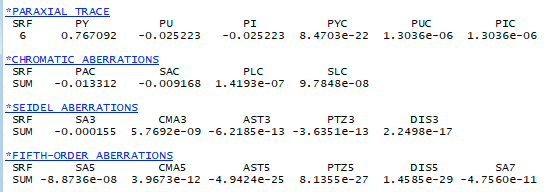
\includegraphics[width=0.59\textwidth]{fotos/AberracionEsf.png} &
            \vspace{0pt} 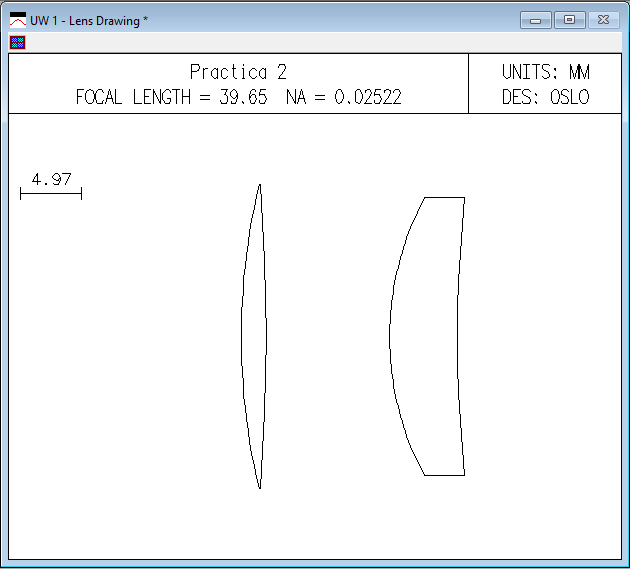
\includegraphics[width=0.39\textwidth]{fotos/AberraciónCorregida.png}
        \end{tabular}
        

\end{document} 